In this section, we will be taking look at the necessary definitions and theoretical fundamentals of various technical terms introduced so far. 
This will help us in understanding the fundamentals of all the concepts used throughout the thesis. We will take a look at the following concepts; 
SceneFun3D tasks and thier importance, 3D scene graphs and their uses, methods for generating scene graphs, semantic and instance segmentation of objects, 
approaches for achieving semantic and instance segmentation, the foundation models used and their rationale, and finally, open-vocabulary obejct detection.

\subsection{SceneFun3D tasks:}
The authors of \cite{scenefun3D} introduce 3 tasks in their paper. The three tasks are:
\begin{compactenum}[1.]
\item	Functionality segmentaion.
\item	Task-driven affordance grounding.
\item	3D motion estimation.
\end{compactenum}
The paper exerts pressure on the fact that these tasks are challenging even with todays advancements in 3D scene understanding
and 3D semantic and instance segmentation and solving the task mentioned above will ensure that the system is capable of 
performing intricate tasks which require manipulating fine-grained functional elements of various objects.
For example, opening a door by turning the door handle. If we breakdown this simple task of opening a door into three parts
and then try to map them to the tasks mentioned above we get, task 1 functionality segmentation resembles segmenting out the door handle 
from the door frame, next task 2 task-driven affordance grounding resembles the association of the text query to the actual 
instance of the door handle which can be turned. And finally with motion estimation we get the direction/motion parameters such as direction, action and angle 
in which the handle needs to be turned. Thus, solving the three tasks effectively ensures that the system will be good at performing daily
tasks as delicately as a human. \\
Figure 1 shows the expected output of all the three tasks. Functionality segmentaton refers to segmenting out the functional interactive 
element from the given scene and annotating it with one of the eight affordance labels defined by \cite{gibson}. Task-driven affordance grounding refers to the task
of associating a text query in the context of the scene to the functional element that can be manipulated for the given text description. Finally, motion estimation
aims to provide the motion parameters that the agent should perform in order to successfully interact with the functional element.

Further, SceneFun3D also provides a well difined dataset of 720 recorded scene from the arkit dataset and various assests for each scene 
to train deep learning models that can tackle these problems. They provide the following assets,RGB-D images, poses, accurate laser scans, 
annotations for each element present in the dataset, motion parameters for each annotation and task description in natural language for every function element.
In our thesis, we aim to beat the baseline results obtained by \citet{scenefun3D} for the first two tasks, namely 
functionality segmentation and task-driven affordance grounding. 

\subsection{3D scene graphs:}
The term scene graph was first introduced in \cite{7298990}, as a novel framework for retrieval of images. Here, the authors designed the scene graph which 
consists of three sub parts, the nodes, the edges and the attributes for each node. First, let us understand the definition of a scene graph and later
look at its evolution to 3D. \\
A scene graph can be defined as a structural representation of a particular scene which captures semantically rich information of the objects in that scene [https://arxiv.org/pdf/2201.00443].
This is done by explicitly modeling the objects, their attributes and the relationship between paired objects as scene in Figure below. (take figure from paper above.)
In short, it is called a “scene graph” because it organizes all this information as a graph: the objects are represented as nodes with their attributes, and the edges between these 
nodes are the relationship between these objects. \\

For a robot to navigate around its environment and interact with the objects in its vicinity, it first needs to have a semantically rich map of its surroundings. 
This surroundings area where the robot can move and interact is called as the scene and the semantically rich map must contain the 
semantic data of all the objects in the scene as well as their locations and inter object realtionships. 
A 3D scene graph can be used to store such a semantically rich data of the objects of the robot’s surroundings. \\

A 3D scene graph is an extension of the traditional scene graph. It is a spatial representation of the objects, their attributes 
and their relationships in three dimensions, in short, they store 3D information. The objects in 3D scene graphs are modelled as
 3D point clouds and they visually resemble the original object. The distinction between a normal scene graph and a 3d scene graph 
 can be seen from the Fig1. 

To further elaborate on 3D scene graphs, consider the example of a scene where a blue water bottle is on top of a wooden table. 
The scene graph here consists of two nodes: 
the first node is the bottle with “blue” as an attribute, and second node is the table with "wooden" as an attribute. The spatial relation, 
"is on top of” is given by an edge. Thus, the scene graph provides a compact representation of the scene to the robot. 
An example can be seen from our implementation in the Fig 2 below.

Uses of 3D Scene Graph:
As we discussed above the scene graph can be leveraged by a robot to navigate around a scene and complete its tasks by manipulating objects defined in the task. 
Apart from this there are numerous other tasks which can be accomplished using either a traditional scene graph or a 3D version of it. 
Scene graphs have been used to enhance image generation [https://arxiv.org/abs/1901.03762, https://arxiv.org/abs/1804.01622], 
the relationships between the nodes are leveraged to incorporate meaningful information during the image generation process to get realistic images.
 Other uses include image captioning using scene graphs 
 [https://openaccess.thecvf.com/content_CVPR_2019/html/Yang_Auto-Encoding_Scene_Graphs_for_Image_Captioning_CVPR_2019_paper.html]. 
 Scene graphs can also be used to detect visual relationships between objects in an image [], Visual question answering, semantic image retrieval and many more.

Before moving to the generation of 3D scene graphs, we will look at the tools used during this process. 
These tools are mainly machine learning and deep learning models. Scene graphs are generated from RGB-D images and poses. 
Out of these, RGB images play an important role in providing semantic information to the scene graph. RGB images are used for object detection,
object segmentation, relationship building and caption generation. All of these tasks are possible due to one or more AI models.
Mainly foundation models like Visual Language Models such as LLaVA and Chat Gpt 4 are used for caption generation and 
relationship building, and SAM for object segmentation. Along with this, object detection models like YoLo form the basis of 
3D scene graph generation. 
Next, let us look at the theoretical concepts behind these models then have a look at how they help in scene graph generation.
\subsection{Foundation models:}
Foundation models can be defined as large-scale, pre-trained models that can perform various downstream tasks\cite{bommasani2022opportunitiesrisksfoundationmodels}. 
Foundation models have two reasons for being successful, scale and transfer learning. On one hand, Scale represents,
more computing power in terms of CPU, GPU and memory and large amount of multimodal training data. Such data is gathered from 
massive datasets generated across diverse domains, this makes generalization possible in foundation models. On the other hand, transfer
learning takes the learnings from one task (e.g., object recognition in images) and
applies it to another task (e.g., activity recognition in videos). 
\begin{figure}[h!]
    \centering
    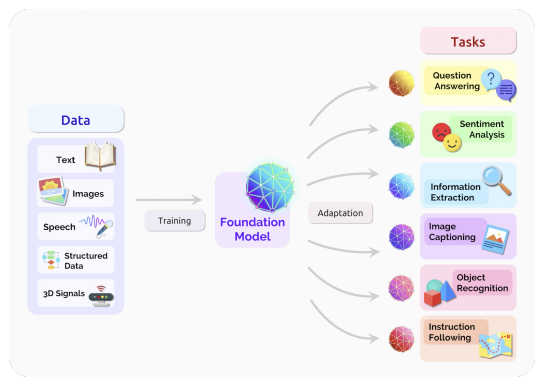
\includegraphics[width=\textwidth]{images/FoundationModels.png}
    \caption{Foundation model overview.}
    \label{fig:foundation_model}
\end{figure}
From \cref{fig:foundation_model} we can see that, 
A foundation model gathers the knowledge from all the data from various data sources such as, texts, images, videos and many more.
This model then adapts to a wide range of downstream tasks such as, question answering, sentimen analysis, object detection just to 
name a few. Their applications range from natural language processing (NLP), computer vision (CV) to robotics and more. 
Let us look at some of the foundation models we will be using in our scene graph implementation.

\subsubsection{Segment Anything model [https://arxiv.org/abs/2304.02643]:}
The paper by \citet{kirillov2023segment} first introduced Segment Anything Model (SAM). SAM is developed by Meta FAIR. 
This foundation model can segment any given 2D image. Segmentation can be made using the following ways, 
it can be prompted with interactive points and boxes, automatically segment everything in the image without a prompt, 
and generate multiple masks for ambiguous prompts. According to Meta AI, “Sam has learned a general notion of what objects are – this understanding enables zero-shot generalization to 
unfamiliar objects and images without requiring additional training.”. The outstanding accomplishments of SAM are possible due to the fact that
the authors used large number of masks approximately 1 billion masks from 11 million images to train the model. Due to such large dataset, 
the model has learnt to segment almost anythin out of a given image, hence the name Segment Anything Model.

\subsubsection{Vision Language Models (VLMs):}
VLMs are advanced machine learning models able to process visual and textual data. 
They  can generate outputs based on the understanding of the multimodal (text and image) input provided to them. 
In this chapter we will be looking at the two most used VLMs, ChatGPT-4 and LLaVA.
ChatGPT-4:
LLava [https://arxiv.org/abs/2304.08485]
 Large Language and Vision Assistant (LLaVA) is an end-to-end large multimodal model trained on data generated with the help of GPT-4. 
 It connects vision encoder and LLM for general purpose visual and language queries. LLaVA performs well on vision queries. 
 Vision queries are queries where the model is provided with an image and a general query is asked regarding the image. 
 For eg, An image with a room is provided and the query can be, ”Is there a computer present in this image?”. 

\subsection{Object segmentation:}
\subsection{Open-vocabulary obejct detection:}
\subsection{Generating scene graphs:}
